
\begin{appendices}

\addtocontents{toc}{\protect\setcounter{tocdepth}{0}}

\chapter{Supplementary Material}

\begin{figure}[ht]
	\begin{center}
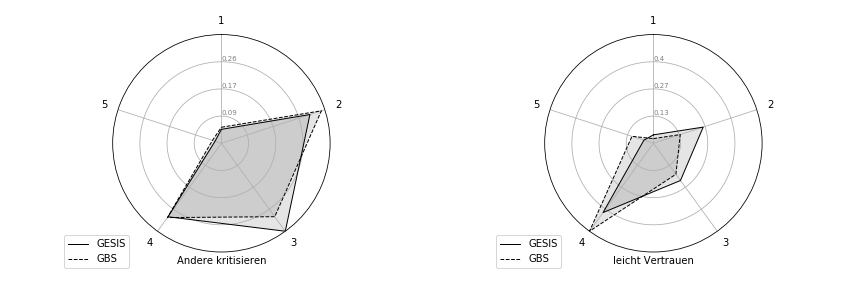
\includegraphics[scale=0.45,angle=0]{fig/Agreeablenessfigure} \\
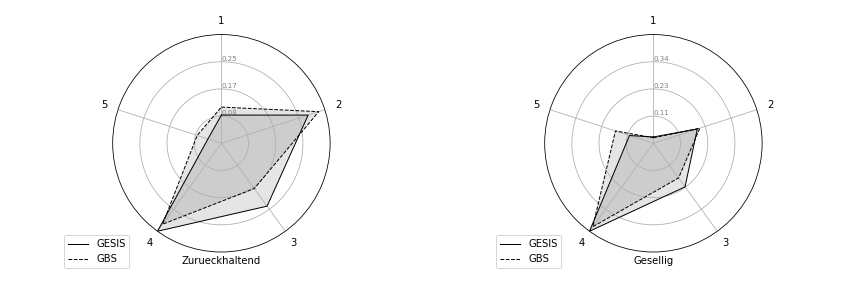
\includegraphics[scale=0.33,angle=0]{fig/Extraversionfigure} \\
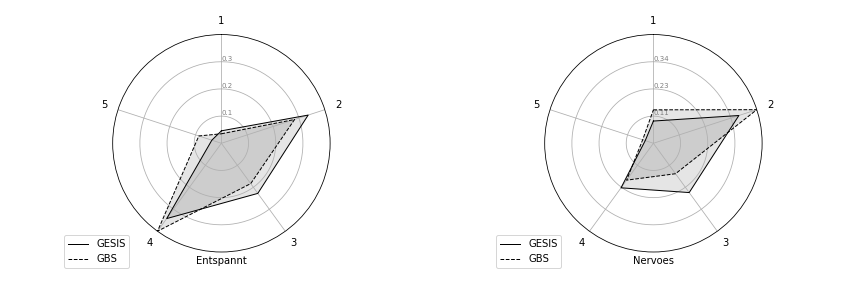
\includegraphics[scale=0.33,angle=0]{fig/Neuroticismfigure} \\
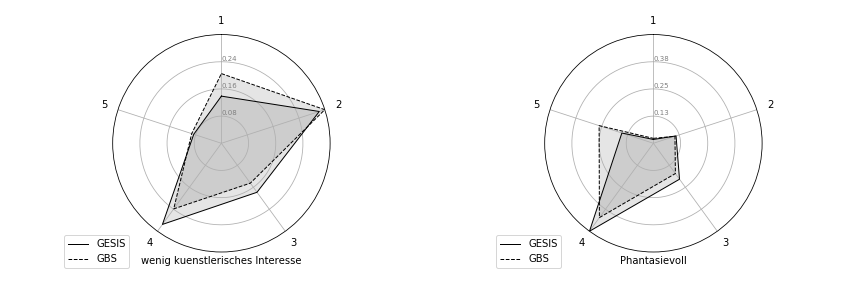
\includegraphics[scale=0.33,angle=0]{fig/Opennessfigure} \\
\caption{Agreeableness is the measure of one's cooperation, empathy, and willingness to trust and help others. Openness estimates whether one is hesitant or eager about new objects or situations. Extraversion refers to level of sociability, seeking and enjoyment of social contact, and energy and assertiveness in social situations. Neuroticism is characterized by easily experiencing negative emotions, and a poor coping response to those emotions. }
\end{center}
\end{figure}

\begin{figure}[h]
	\begin{center}
		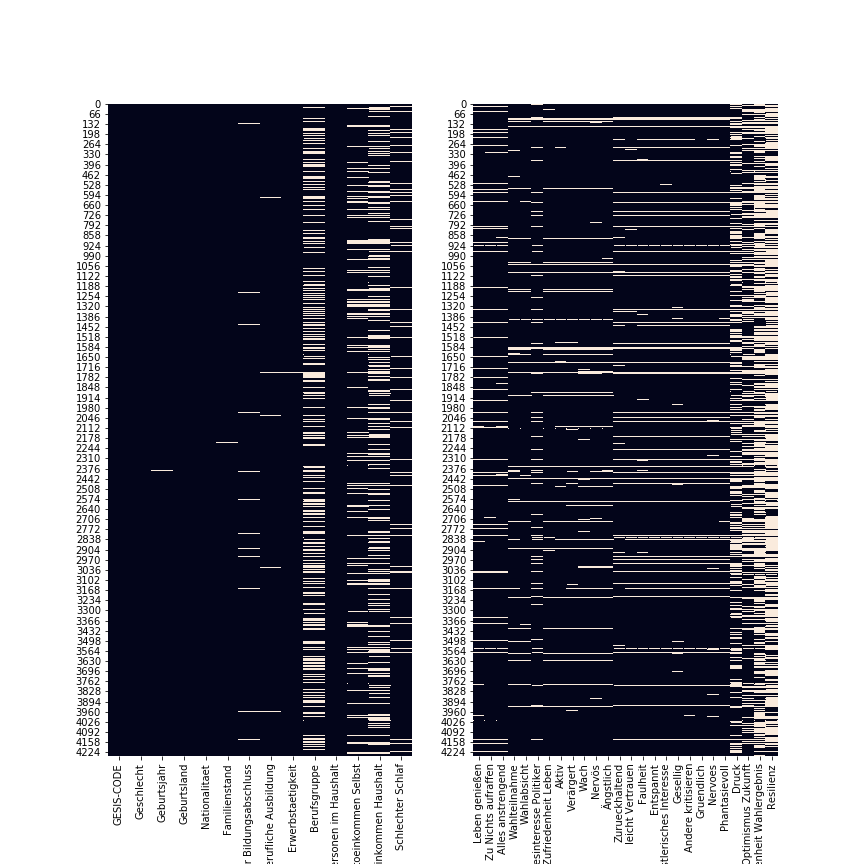
\includegraphics[scale=0.50,angle=0]{fig/gesis_missing}
		\label{std}
		\caption{The attribute values of a participant are always known for "Geschlecht", "Geburtsland", "Geburtsjahr", "Nationalitaet", "Familienstand", "Personen im Haushalt". In contrast, the last three columns "Druck", "Optimismus Zukunft", "Zufriedenheit Wahlergebnisse" and "Resilienz" are almost always missing and are therefore removed from the analysis. Participants with missing BFI-10 elements are removed. Sample size will only be reduced slightly as missing values often occur for the same instance. These dependencies form a line pattern in the graph. "Berufsgruppe" was surveyed as a text field so that the column clearly suffers from ambiguous value mismatch. To include "Berufsgruppe" mappings need to be redefined first. For now, "Berufsgruppe" is removed. }
	\end{center}
\end{figure}

\begin{figure}[ht]
	\begin{center}
		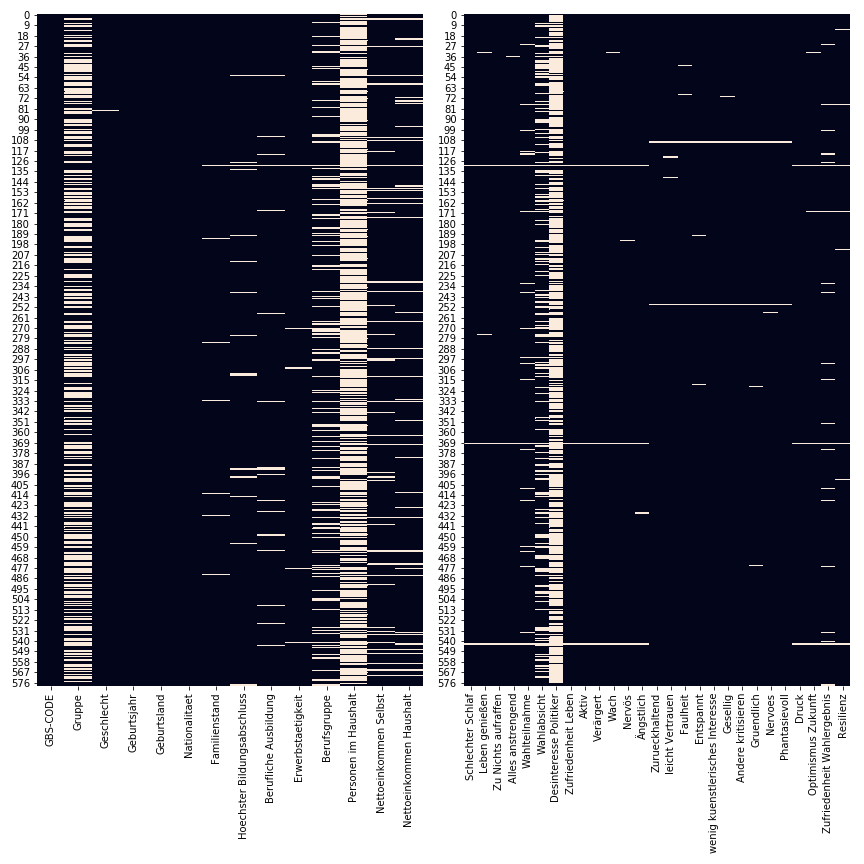
\includegraphics[scale=0.50,angle=0]{fig/gbs_missing}
		\label{std}
		\caption{There is one more attribute in "Gruppe". Not every participant received a positive a negative psychological treatment. Therefore, "Gruppe" is more likely to be missing than not. However, the absence of a value indicates no treatment rather than a missing positive or negative. "Gruppe" is not properly represented yet. "Desinteresse Politiker" is given by multiple data sources from different excel files. Some of them being the inverse of the attribute itself. The surey design regarding this issue is unclear to me. To incorporate "Desinteresse Politiker" the attribute(s) need to be imported correctly, if possible. Another import issue is given by "Personen im Haushalt". If the actual value is greater than one, the cell will be empty. To correct this, the corresponding csv-file needs to be fixed. The text field "Berufsgruppe" suffers on both ends, GBS and GESIS, due to current oversimplification of value and potential data mismatch.}
	\end{center}
\end{figure}

\begin{figure}[ht]
	\begin{center}
		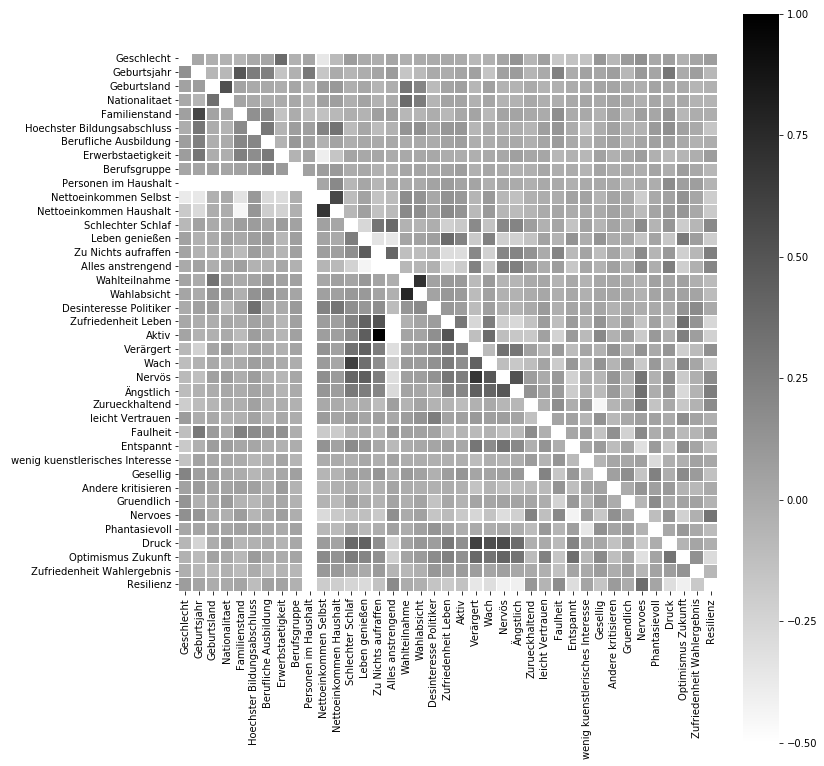
\includegraphics[scale=0.73,angle=0]{fig/correl}
		\label{std}
		\caption{The upper right triangular matrix shows GESIS correlations while GBS correlations are shown in the lower left. The main diagonal should not be confused with white squares. These trivial combinations are simply excluded and not colored black. As can be seen "Personen im Haushalt" in GBS can not be calculated, since there is only one possible value. "Nettoeinkommen Selbst" and "Nettoeinkommen Haushalt" are highly correlated but not removed or handled at all. I will keep this in mind, when facing the naive bayes assumption in the learning process. Entropy-based mutual information in "Wahlteilnahme" and "Wahlabsicht" have led to almost perfect classification performances in predicting political participation. "Wahlabsicht" is therefore removed.}
	\end{center}
\end{figure}

%\begin{figure}[ht]
%	\begin{center}
%		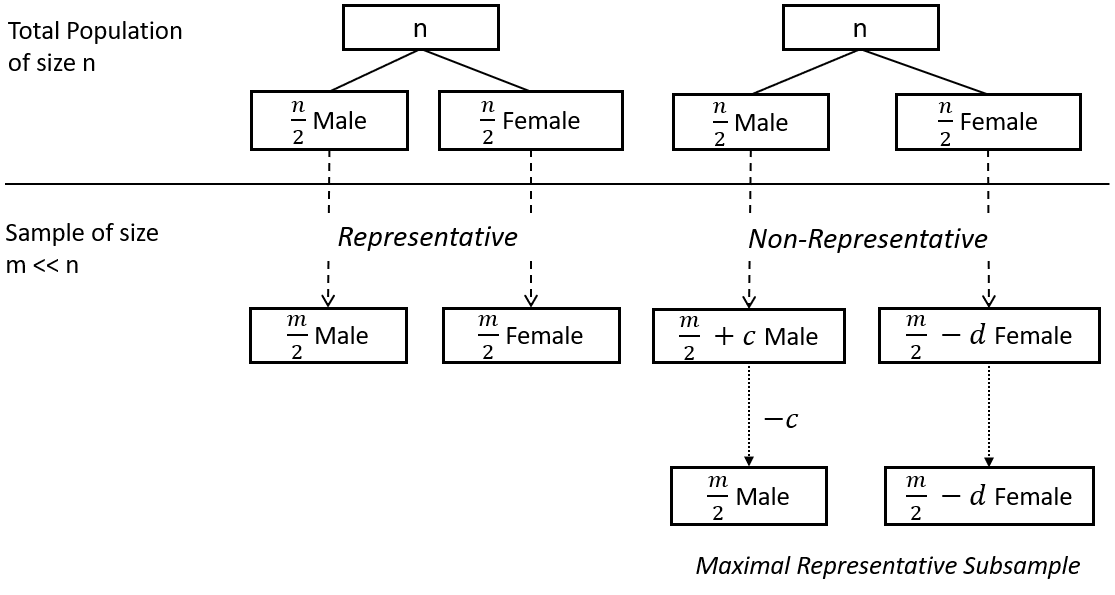
\includegraphics[scale=0.40,angle=0]{fig/Representative}
%		\label{representativ}
%		\caption{Consider samples of fixed size \(m\) with some constants \(c_m\) and \(d_m\). Maximal representative sampling adjusts for nonresponse \(-d\) of subgroup \(Female\) %by removing \(+d\) of subgroup \(Male\) from the sample.}
%	\end{center}
%\end{figure}

\chapter{GitHub Repository}

\begin{figure}[ht]
	\begin{center}
		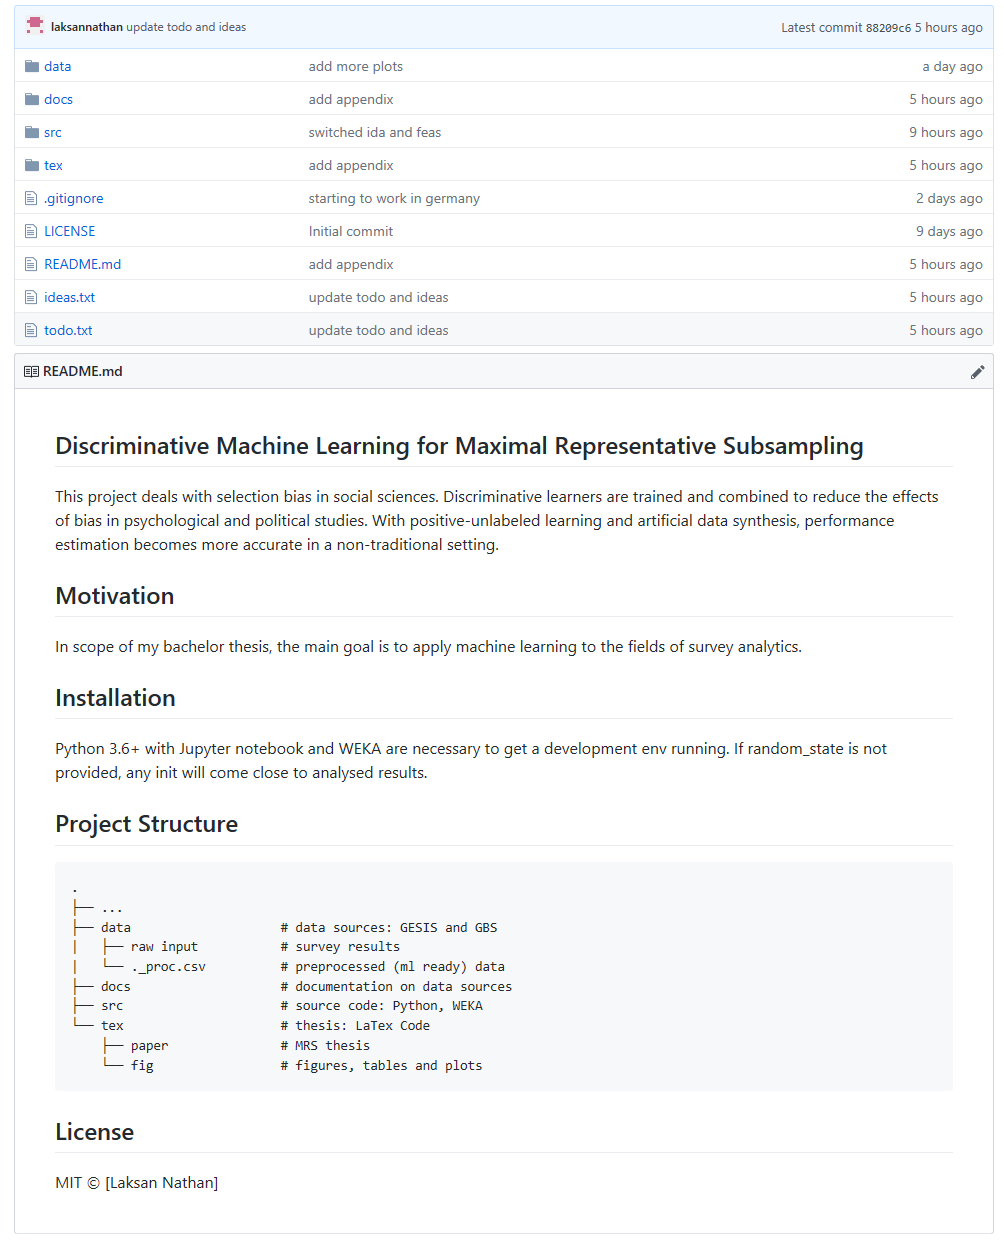
\includegraphics[scale=0.48,angle=0]{fig/github}
		\label{std}
\caption{The upper right triangular matrix  "erformances in predicting political participation. "Wahlabsicht" is therefore removed.}
	\end{center}
\end{figure}

%\newpage
%\pythonexternal{fig/latex.py}

\end{appendices}